\documentclass[a4paper,12pt]{article}

% removed all the \ifx \pdfoutput stuff as we are using pdflatex and we are embedding only png images.. forget the old ecs files !!!
\usepackage{graphicx}
%\usepackage{epstopdf}

\usepackage[english]{babel}
\usepackage{ucs}               % require separate debian package 
\usepackage[utf8x]{inputenc}   % require ucs. Allows both Italian and English letters.
\usepackage[T1]{fontenc}
\usepackage{fancyhdr}
\usepackage{subfigure}
\usepackage{amssymb,amsmath}
\usepackage{threeparttable}
\usepackage{color}
\usepackage{url}
\usepackage{natbib}  % substituted hardvard with natbib as the former package doesn't like the hyperref one
\usepackage{rotating} %to have text vertical alignment in some table headers
\usepackage{url}
\usepackage{moreverb}

\usepackage{html,htmllist} % don't think will be needed

%\usepackage{../autogeneratedDoc/latex/doxygen}

% If I uncomment the following line I get nice links in the PDF but long
% links don't get brooked in the bibliography :-(( :
%\RequirePackage[plainpages=false, colorlinks=false, draft=false]{hyperref} %setting draft=false will create the table of content in AcroBat with all the internal links as well (surrounded by a coloured box)
%\def\pdfBorderAttrs{/Border [0 0 0] } % No border arround Links
%\usepackage[plainpages=false, colorlinks=false]{hyperref}
\usepackage{hyperref}

\bibliographystyle{agsmurl}  % bibliographic style


% increase the horizontal text space...
\addtolength{\hoffset}{-0.5cm}
\addtolength{\textwidth}{1cm}
\addtolength{\voffset}{-1cm}
\addtolength{\textheight}{2cm}
\setlength{\headheight}{14.5pt}
%\addtolength{\oddsidemargin}{1.6cm}    %otherwise the odd pages have higher right margin and the opposte.. strange!!!!
%\addtolength{\evensidemargin}{-1.6cm}

% headers and footers...
\pagestyle{fancy}
\fancyhf{}
\fancyhead[RO,LE]{\textit{\leftmark}}
\fancyhead[RE,LO]{RegMAS User Manual}
\fancyfoot[RO,LE]{\thepage}
\renewcommand{\headrulewidth}{0.4pt}
\addtolength{\headheight}{0.4pt}
\renewcommand{\sectionmark}[1]{\markboth{#1}{}}
\renewcommand{\subsectionmark}[1]{\markright{\thesection\ #1}}


%opening
\title{RegMAS User Manual\\
\begin{scriptsize}\textit{Version 1.3.0}\end{scriptsize}
}
\author{Antonello Lobianco\footnotemark[0] \footnote{Department of Economics, Marche Polytechnic University.} \footnote{I want to thanks Roberto Esposti for his precious directions, Franco Sotte and the Department Of Economics at UNIVPM for funding this project and Alfons Ballmann, Kathrin Happe and the whole IAMO team (Konrad, Christoph, Martin..) for their AgriPoliS model from which RegMAS has borrowed many concepts and their support in my studies of agent-based modelling.} }
%\affiliation{UNIVPM}
%\email{a.lobianco@univpm.it}   %optional
\date{
September 30, 2008
\begin{figure}[!hbp]
	\centering
	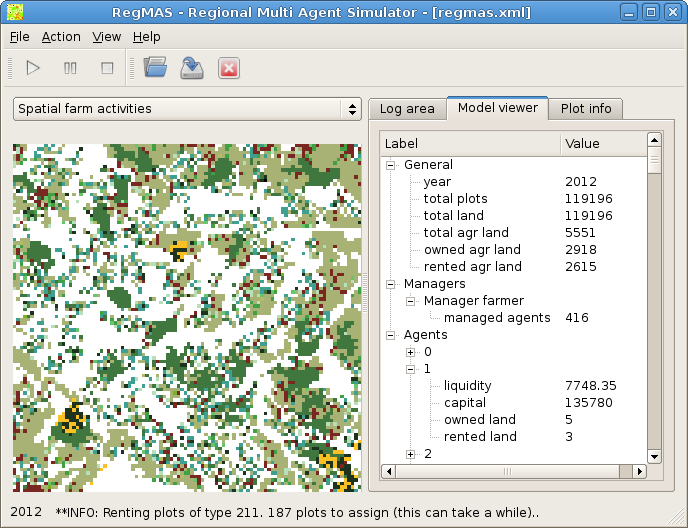
\includegraphics[width=0.6\textwidth]{imgs/screenshots/mainWindowPlain}
	\label{fig:mainScreenshot}
\end{figure}
%\vspace*{1cm}
}
\begin{document}
\maketitle


\begin{abstract}
RegMAS (Regional Multi Agent Simulator) is a spatially explicit multi-agent model framework, developed in C++ language and designed for long-term simulations of government policies effects over agricultural systems (e.g. farm sizes, incomes, land use).

RegMAS uses a profit-maximisation algorithm to derive farmers behaviours. Using RegMAS researchers can write regional-specific models, adapting the pool of activities and resources to their specific region.

RegMAS is \textit{Free Software}, that is, its source code is fully available and modifiable, and it runs on several operating systems.

This paper is designed to introduce RegMAS and to assist researchers in using it for their own simulations.

\end{abstract}

\thispagestyle{empty}

\newpage
\tableofcontents
\thispagestyle{empty}

\newpage

\section{Introduction}

While many and heterogeneous models exist nowadays to assess the impact of government policies or market rules over agricultural systems, very few (if any) address the basic concerns of the academic community of transparency and reproducibility of experiments. Instead, most times the reader must be satisfied with validation experiments conducted by the researchers themselves.

To address this needs, we chose to develop our own model as \textit{Free Software}, that is, its source code is publicly available and can be freely used and modified.

RegMAS (Regional Multi Agent Simulator) is a spatially explicit multi-agent model framework, developed in C++ language designed for long-term simulations of effects of government policies on agricultural systems (farm sizes, incomes, land use..).

More specifically, RegMAS conceives rural social systems (and in particular agricultural ones) as complex evolving systems, made of an heterogeneous set of individual acting ``agents'' (that is, farmers).

The researcher typically set the initial conditions where the farmers operate and ``observe'' their behaviours in such environment. Initial conditions can include pre-defined shocks along the temporal dimension, typically used to model changes in the policy or macro-economic variables (e.g. decoupling options, activities gross margins..).

This document will help you discover RegMAS and hopefully will make your life easier while using it for your own simulation exercises.

It is structured as follow.

Section \ref{sec:methodology} briefly describes the history and the methodology behind RegMAS, referring for details on several papers that discuss multi-agent models applied on agricultural systems.

Section \ref{sec:installation} will guides users from obtaining the program with associated sample data trough having it working on their pc. It covers a typical MS Windows installation, while the compilation of RegMAS directly from the source code is covered in a corresponding section on its web-site wiki.

Once the program is installed, sections \ref{sec:predefined_scenarios} to \ref{sec:programming} will gradually introduces in the usage of RegMAS. Section \ref{sec:predefined_scenarios} presents the program user's interface and the input files, allowing to run a complete RegMAS experiment using the predefined scenarios over the sample data. Users interested in creating their own scenario should consult section  \ref{sec:new_scenarios}. A further point that most RegMAS users will likely be interested is how to apply the model over their own case-study region. This requires obtaining farm-specific and regional-level data (including spatial one) and it is covered on section \ref{sec:new_region}.

Finally some researcher may want to personalise RegMAS, maybe changing the farmers behaviours or adding new details to the output. As previously noted, source code of RegMAS is fully available and users are encouraged to modify it for their own modelling needs. Section \ref{sec:programming} gives a brief tour of the RegMAS Application Programming Interface (API), presents the tools used to develop RegMAS and point on the specific place where to get more help.

Once a user has became familiar on creating new scenarios or models, it will be time to analyse the results. Sections \ref{sec:results} and \ref{sec:gis} respectively describe the kind of results that are saved by RegMAS and how to export them into a GIS for further analysis (the latter task is optional but recommended).

This manual ends with an Appendix covering the sources where further help in using RegMAS may be available and the license terms.

Have fun with RegMAS !


\section{The model}
\label{sec:methodology}


\subsection{Overview}

Spatial explicit Agent-Based Models (ABM) within the specific agricultural context was pioneered by \cite{Balmann:1997} with the Agricultural Policy Simulator (AgriPoliS) model.

ABM have the benefit of catching the fundamental behaviour at the micro-level of the individuals farms, without the need of aggregating them in ``representative'' agents. Maybe even more important, ABM can catch the iterations of the heterogeneous farms when they deal with competition over common finite resources, e.g. land.

\cite{Boero:2006} and \cite{Parker:2003} have review several other ABM involving land use changes in various scientific areas, including agricultural economics, natural resource management, archaeology and urban simulation, but this section will briefly describes AgriPoliS as RegMAS borrows many concepts from it, \textit{in primis} the utilisation of a profit-maximisation algorithm to derive farmers behaviours.

AgriPoliS allows to model heterogeneous farms behaviours under various external situations (typically, under different policy scenarios) and observe regional results by aggregating these micro-level behaviours.

In AgriPoliS agents are mainly farmers\footnote{Other agents in the model perform some specific tasks, e.g. managing land or coordinating product markets.}.
They have their own goals; in AgriPoliS, the farmer's objective is the maximisation of household income.
To achieve this objective, farmers solve a Mixed Integer Programming (MIP) problem that, in some aspects, is specific to each farmer.
Outside the linear programming problem, they can also decide to rent other agricultural plots or to release rented land.

Using a mixed integer linear programming approach to simulate each agent behaviour on one hand is very flexible, as it can cover the whole range of farm activities, from growing specific crops to investing in new machinery or hiring new labour units.
Furthermore, it is simple to add new regional-specific activities.

On the other hand, however, linear programming techniques require a long calibration phase to assure a balanced choice of farm activities, avoiding unrealistic outcomes \footnote{RegMAS introduces a sub-region mode to help researchers to roughly calibrate their model before running a real (and slower) simulation.}.

Any farmer in the model is a real farmer whose data are taken from farm-level datasets (in Europe, FADN) and explicitly associated to a spatial location.
Due to privacy-protection regulations, however, we don't have access to the real farm localisation.
Therefore, we have to distribute farms randomly in the virtual region. Space (i.e. location) is important in the model because it influences transport costs and indirectly makes the farmers interact each other, e.g. by competing for the same land plots.

AgriPolis, as it takes into account many aspects of a real farm, is a very complex model, with lot of code dedicated to cover specific aspects (e.g. quotas, generational changes, multi-years investments). A detailed description of AgriPolis can be found in \cite{Happe:2004} or in \cite{Kellermann:2007}.
While \cite{Happe:2004} focus is on the methodological advantage of using ABM in agriculture as compared with other instruments as partial and general equilibrium models on one side and individual farm-level models on the other, \cite{Kellermann:2007} details the latest implementation of AgriPoliS (2.0).
In addiction to this two papers, \cite{Sahrbacher:2005} describes AgriPoliS implementation over several case-study regions and \cite{Lobianco:2007} presents an adaptation of AgriPoliS for the Mediterranean regions, further adding some general background on agent-based modelling and to its motivations.

\medskip 

As AgriPoliS, RegMAS is spatially explicit, a characteristic that can not be neglected when modelling the agricultural sector. For example the spatial heterogeneity allows the model to associate on each plot a different rental price and investigate possible land abandonment phenomenas even when the land is \textit{on average} profitable.

Differently from AgriPoliS, the spatial dimension is initialized from real land-use data, using satellite information, and plots are explicitly modeled in the decision matrix as individual resources.

As a further distinction, RegMAS has been designed from the ground-up to explicitly consider farmers as one type of several possible type of agents. In RegMAS farmers have sensitivity of the overall environment, including extra-agricultural variables. On a technical point, ``farmer'' agents in RegMAS derive from a more general type of ''spatial`` agents that in turn derive from a ''base`` type.
Each agent type has its own ''manager`` agent that dialogue with a ''Super Agent Manager``. The formers are a sort of interface ''agent side`` while the latter implements the same interface on the program core side. In this way the model core doesn't need to know anything about agents internal logic.
While this approach allows for rapid development of different agent types (only specific characteristics need to be modelled) at current RegMAS development stage only farmer agents are fully implemented.

\subsection{Farmer agents behaviour}
\label{sec:methodology:farmers_behaviour}

Farmers autonomously make their decisions solving a Mixed Integer Programming (MIP) problem similar to those shown in Figure \ref{fig:mipSample}.
This happens any time farmers bid for renting a land plot in order to calculate its shadow price, or plan for new investments, or finally produce using the given assets.
Symbol 
\includegraphics[width=15px]{imgs/mipSymbol} in Figure \ref{fig:flowchart} denotes a step in the model when one or more MIP problems have to be computed at the farm level.

\begin{figure}[!hbp]
	\centering
	\caption{Agent's Mixed Integer Programming Problem (excerpt)}
	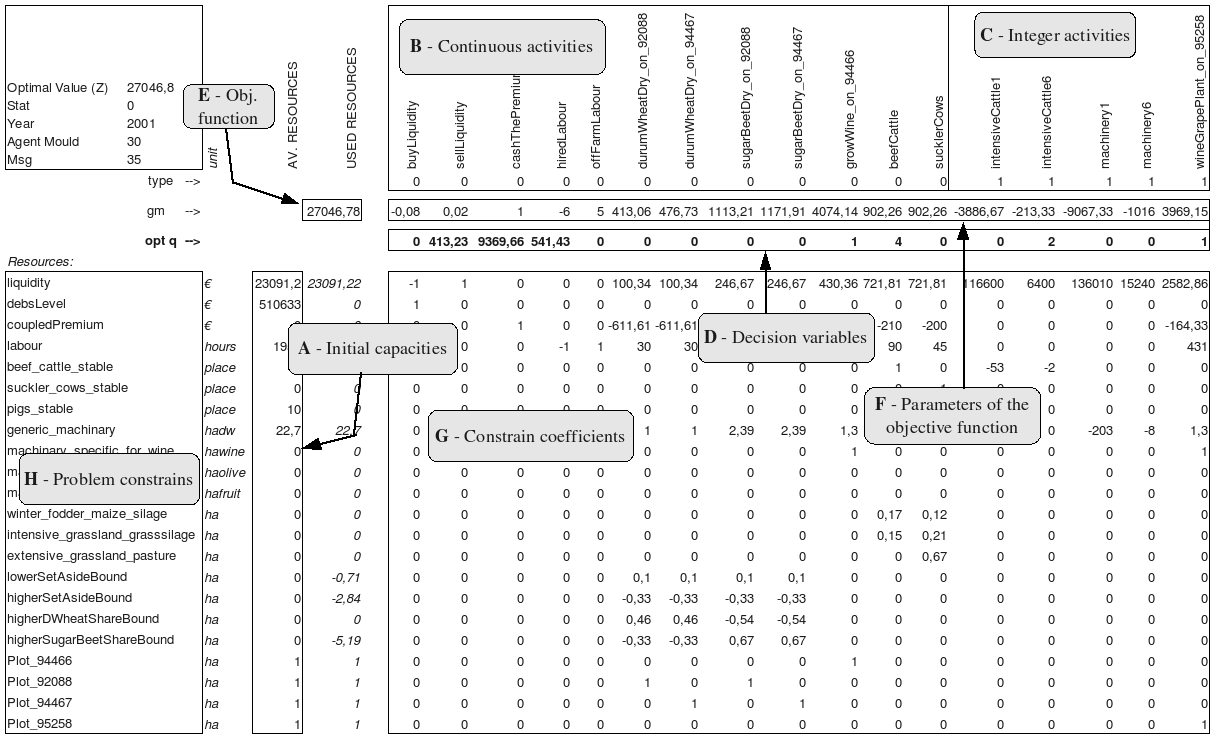
\includegraphics[angle=90,width=0.95\textwidth]{imgs/mipSample}
	\label{fig:mipSample}
\end{figure}

\begin{figure}[!h]
	\centering
	\caption{RegMAS general Flowchart}
	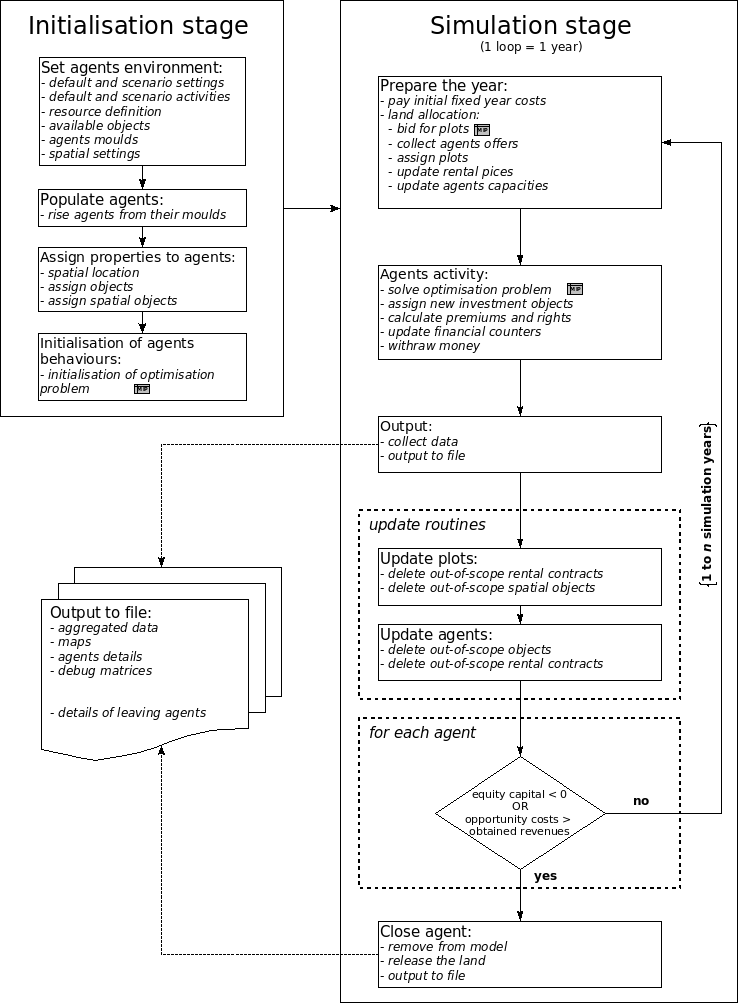
\includegraphics[width=\textwidth]{imgs/regmasFlowChart}
	\label{fig:flowchart}
\end{figure}


From FADN data we can establish the initial farm's endowment: financial assets, availability of land, machinery, animals and so on.
From a linear programming point of view, these data represent the right terms of the constrain equations (A in the cited figure).
Any farmer choose from a list of activity options.
They can be divided in two categories: activities that can be run entirely within one year (B) and activities that generate results over multiple years (investments, C).
Investments are bounded to be integer and the same investment type is available in different size-options, allowing scale-effects to emerge in the model. Section \ref{sec:methodology:farmers_behaviour:finance} details the farmers finance modelling, including how investments enter the MIP together with yearly activities.

Individual activities to include in the model are left to the RegMAS users. Currently we implemented models where, very synthetically, all aspects of running a farm are considered, including financial and labour ones.
To solve this problem the farmers chose the quantities (D) of the various activities that maximise the objective function (E).
In our case, this is the maximisation of household income, and the gross margins of the various activities are the parameters of the objective functions(F).

Before entering the MIP, individual activies are ''filtered`` by the farmers. Currently, this is implemented in order to change the gross margins to include transport costs from the farmstead to the plot and to take into account the plot's altitude (under the hypothesis that mountain plots are less productive than plain ones).
Finally, The matrix of the constraint coefficients (G) links the available activities (B+C) with their technical requirements (H).

RegMAS can take into account changes of resource endowment and activity gross margins, generated either endogenously to the MIP core, in case these changes occur as a consequence of the solving procedure (e.g., an investment improves the number of available activities) or exogenously to it, in case these changes occur in other parts of the model (e.g., renting/releasing land, or as a consequence of market prices changes).

\cite{Paris:1991, Arfini:2000} present respectively an in-deep analytical description and a literature review of linear programming techniques applied to farm problems.



%As example, our preliminary results shown how changes in agricultural policies affects differently areas that are fully agricultural from areas where agricultural activity is dipped in a matrix composed of other activities (e.g. natural vegetation or urban use) where distances become higher.

%Finally the spacial dimension in RegMAS is \textit{fully} explicit, and initialized from real land-use data, using satellite informations. Plots are explicitly modeled in the MIP as individual resources, while in AgriPoliS they are aggregated according to their land type (e.g. under the resource “arable land”). Aside the opportunity of seeing where production happen, this implementation leads to easy improvements of the model over other layers of spacial information. E.g. it is relatively easy to insert an information about altimetry that influences individual plots revenue capacity.

%Few paragraphs on RegMAS, history (AgriPoliS, bibliographical notes, ), multi-agent methodology, strong and weak points. Getting them from the PhD thesis. 

\subsubsection{The space dimension in the optimisation problem}
As result of the spatial explicitness the farmer maximisation problem is composed of the following activities:
\begin{itemize}
 \item $i$ spacial explicit activities * $p_i$ suitable plots;
 \item $j$ spacial explicit investments * $p_j$ suitable plots;
 \item $q$ other spacial implicit activities;
 \item $z$ other spacial implicit investments.
\end{itemize}

Is the researcher task to select which characteristics need to have a plot to be considered for each spatial explicit activity.
Within the input data, he/she can select which land types and even which spatial objects need to be already present for each activity.
To make an example, growing wine requires land type \textbf{221} (vineyards) and the presence of a \textbf{wineGrapePlant} object.
All \textit{activity\_x\_plot} combination that miss this requirements are automatically discarded even before entering the MIP, reducing the MIP dimension and therefore the required computational power \footnote{The Reference Manual has a pseudo-code that details the steps the model does to add activities to the MIP problem, available at \url{http://regmas.org/doc/referenceManual/html/classOpt.html}.}.

Even with this trick, the spacial explicitness has the disadvantage of a much larger matrix, especially in case of farmers with many plots, but it has also many advantages:
\begin{itemize}
 \item transport costs are associated directly with individual pixels and already included in the Gross Margin;
 \item pixel heterogeneity (e.g. different slopes) can be included straightforward, just changing the gross margins (e.g. through the ''filter`` function cited in the previous section);
 \item an explicit map of the region can be draw to show the different productions;
 \item binds on individual plots can be easily inserted on the MIP problem.
\end{itemize}

\subsubsection{Financial aspects}
\label{sec:methodology:farmers_behaviour:finance}

In RegMAS models investments require liquidity that can be obtained using open-credit line that can grow up to a model-fixed share of the capital (e.g. 80%).

Each year the farmer optimize the quantity of money to ask to the bank. There isn't an end-term for farmers to give back the money as the ''bound`` is rather as the debit share of the capital.

Differently from AgriPoliS there is no difference from short-term loans and long-terms one. This is because loans are completely decoupled from investments. On the other side, there is no needs to assume a constant share of investment covered by the loan: the individual farmers are free to implicitly optimize the share of the investments covered by loans depending on their financial situation.

Liquidity is calculated as follow:

\begin{eqnarray}
\label{eq:liquidity}
liquidity_t & = & liquidity_{t-1}+profits_{t-1} \nonumber \\
            &   & -withdraws_{t-1}-\sum_{n=0}^{N}{invCosts_{t-1,n}}-sunkCosts_{t}
\end{eqnarray}

To calulate the liquidity available to farmers on a specific year we sum to the liquidity available on the previous year all the revenues (profits) and costs (withdraws and new investments) occurred in the previous year and we detract the sunk costs farmers need to pay before producing (these are costs generated from prevoius choices, like multi-year rental costs or investment maintenance costs).

Withdraws are the money required by the farmers to support their own private life. They are calculated as a fixed portion of the profits plus a minimum level that depends from the size of the farm (misured in family annual work units):

\begin{eqnarray}
\label{eq:withdraws}
  withdraws & = & perCapMinWithdrawal*AWU \nonumber \\
     &  & + max(0,profits*withdrawalProfitShare)
\end{eqnarray}


If the liquidy can be tought as a buffer, the debit level shoud be considered as a threshold, expressed as the share of the whole capital that farmers can't overpass.

The whole capital is in turn calculated as the sum of the liquidity, the investments current value and the land capital:

\begin{equation}
\label{eq:capital}
capital_{t}=liquidity_t+ \sum_{i=0}^{I}{investmentCurrentValue_{i,t}}+landCapital
\end{equation}

with $I$ is the number of owned investments. The current value of investment objects depends from the kind of investment itself: e.g. in perennial crops the value first grows up and then decreases, in stables instead it linearly decreases.\\
$landCapital$ is, at least now, fixed and read from the farmers' data file.\\

\subsubsection{MIP solver}

In RegMAS MIP problems have to be computed for each individual farm and in several steps during each simulated period, resulting in levels of thousands computations for period.
It follows that the speed of the solving algorithm become a critical factor. Due the fact that in RegMAS plots enter the problem individually, matrices can become quite large, however they are very sparse allowing specialised software to solve the problems in terms of fractions of second.

In fact, RegMAS use external libraries to solve this problems. RegMAS class \textbf{Opt()} is responsible to establish the direction of the objective function (in our case, a maximisation), the set of bounds, objective coefficients and constrain coefficients. At this point the problem ``object'' is solved calling an external Dynamically Linked Library (DLL).

RegMAS uses the open-source GNU Linear Programming Kit (GLPK) \cite[]{Makhorin:2007} that employs a two-phase revised Simplex method (that is guaranteed to find the optimal solution, if one exist) to retrieve continuous solutions, and then apply a Branch \& Bound method in case of an integer optimisation.

GLPK recently added an interior-point algorithm, but we found it to be still too unstable at this time.


\subsection{Land allocation and land market}
\label{sec:methodology:land}

An obvious problem when dealing with spatially explicit agent based models is the localisation of the agents and of their spatial objects. The problem is complicated by the fact that there is already an informative layer, consisting of the land use, and we have to keep this layer consistent with the model, applying the farm allocation over it.

Firstly, farms are assigned a random location picking up a plot compatible with their assets, starting from the less common. The idea is that rare land use types have the precedence over common land use types to minimize distances from them to the farmsteads. So if a farm has both fruit land and arable land, the farmstead will be placed within a fruit land type.

Subsequently, plots are assigned to the closest farm that has still an uncompleted capacity for that specific soil type, giving precedence to owner plots in comparison to rented ones.

This is not a optimization algorithm as plots are not assigned to farms in a way that minimize the total plots-farmsteads distance. But on the other hand also the real world situation is far from an optimal land (de)fragmentation, as physical bounds and hereditary rules often split the farmer land in various disconnected plots. Figure \ref{fig:ownedPlots} shows the result of the initial land allocation, with the plots assigned to their owner farm (each colour represent a different farm).

\begin{figure}[!hbp]
	\centering
	\caption{Owned plots after initial land allocation.}
	
\includegraphics[width=0.5\textwidth]{imgs/ownedPlots}
	\label{fig:ownedPlots}
\end{figure}


During the simulation farmers can bid to rent new plots. Currently (as in AgriPoliS) RegMAS doesn't allow for land transfer nor for direct \textit{farmer-to-farmer} renting contracts.  Instead, farmers can only rent land owned by an anonymous agent that collect the land arising from farms leaving the model and from the initial pool of rented plots to make it available in a bid to the farmer offering the highest price.

Farmers asked to bid offer a share of their shadow price for such plot, to take into account of fixed and variable negotiation costs and overheads. The shadow price for the new plot is calculated simply performing two MIP problem optimisation, with and without the plot, and calculating the difference.

While AgriPoliS can use some optimisation techniques as land is homogeneous within the same soil type, the full heterogeneity of plots in RegMAS prevent using such tricks, making this process very computationally intensive.
Therefore RegMAS offer the option to limit the bidding process to farmers within a certain range from the plot.
The natural trade-off when increasing this option is on one side that it increases the likelyhood to get the highest bid, but on the other side that it dramatically increases the computational time.

Once the plot is assigned to a farm a rental contract is established for a random period (within user defined limits) and the plot enter the farmer's MIP problem as a new resource.


\section{Installing RegMAS}
\label{sec:installation}

\subsection{System requirements}

While RegMAS doesn't have many software requirements (it currently run on any PC with MS Windows or Linux \footnote{As RegMAS is written in standard C++ and its dependent libraries are know to work with Macintosh, a Mac port should be easy, ideally just a compilation. However we don't have any experience on such platform and therefore we can not offer assistance on such platform.}), its hardware requirements are of much more constrain.

It will make a severe trial of a pc's CPU and RAM. Exactly how much RAM it needs will depends on the size of the region. For very tiny regions (let's say 50x50 pixels) 256 or 384 MB may be enough, but for a larger region (e.g. 300x300 pixels) we recommend at least 2 GB of RAM. Even in such case a 15 years simulation will last a few hours.

\subsection{Getting the software}

RegMAS can be download in two forms: as a Windows installer or as source-code that requires compilation before it can be used.

The latter form is suggested for users that want to adapt the model to their own needs, or that use Linux (our development environment, for which an installer is not available) or yet that need the very latest version. In such cases the source code can be downloaded directly from our Concurrent Version System (CVS) and compiled, as directed from an apposite page on the documentation wiki.

In all other cases the suggested way is to download the installer\footnote{\url{http://www.regmas.org/download}} and keep reading this section.

A local installation of OpenOffice\footnote{\url{http://www.openoffice.org}}, a free and multi platform MS Office clone suit, is required to edit the input data. In fact, while OpenOffice is not strictly needed lo load the data, from RegMAS version 1.2.0 onward input data is read directly from an OpenDocument Spreadsheet file that can be handled with OpenOffice Calc.

Users can refer to the OpenOffice web-site for directions on how to download and install OpenOffice.

\subsection{Installing the software}
The Windows installation wizard let users decide witch components of the software should be installed (Fig. \ref{fig:installer}). Aside to the main program, also the run-time libraries should be installed, as they are required to run RegMAS.
\begin{figure}[!h]
	\centering
	\caption{Component selection during installation wizard}
	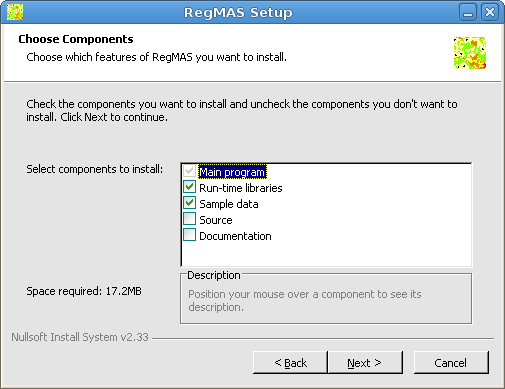
\includegraphics[width=0.8\textwidth]{imgs/screenshots/installer_componetSelection}
	\label{fig:installer}
\end{figure}
Sample data are suggested in order to test the software before building a different model.

Finally, users may want to include the source code and a local copy of the documentation. While unnecessary to run the model, the model code is very useful in order to deeply understand the model behaviour.

\section{Running default scenarios}
\label{sec:predefined_scenarios}
Once the installation is completed RegMAS can be started from its shortcut under $Start Menu\rightarrow Programs\rightarrow RegMAS\rightarrow Version$ or clicking directly on regmas.exe using Explorer.

\subsection{The Graphical User Interface}
Figure \ref{fig:gui} shows RegMAS Graphical User Interface (GUI). It is logically divided into 3 areas.

\begin{figure}[!h]
	\centering
	\caption{RegMAS Graphical User Interface}
	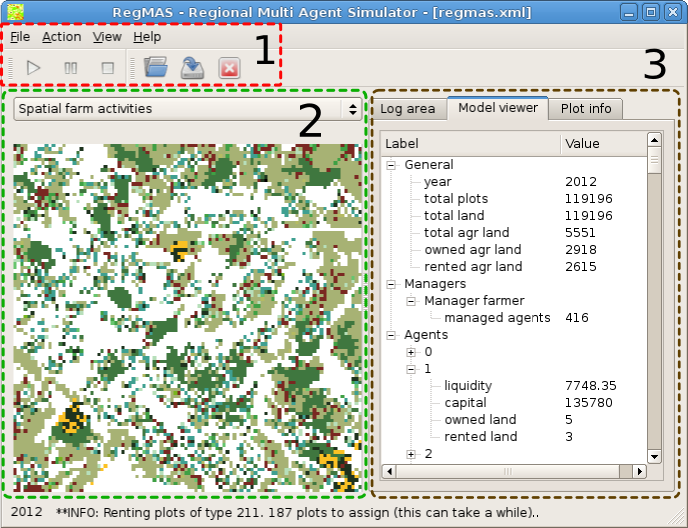
\includegraphics[width=1\textwidth]{imgs/screenshots/mainWindow}
	\label{fig:gui}
\end{figure}

The first area includes the COMMANDS, divided into the \textit{action} toolbar and the \textit{file} toolbar. From left to right, they allow to \textit{run} the model, to \textit{pause} it, to permanently \textit{stop} the model, to \textit{load} a new model, to \textit{save} a model log and finally to \textit{exit} the program.

Even if we checked the code very accurately, it is not advisable to run several simulations consecutively. This because memory leaks are likely to arise and in the worst scenario to interfere with the model. Instead, users can close the program and re-open it at each newer simulation.

The second area displays the MAPS (spatial layers) that are loaded or drawn by the model. They are upgraded at least once for each simulation year, and are the quickest way to see what it is happening on the model during run-time. Layers can be switched using the drop-down menu at their top and can be zoomed or scrolled using the mouse. Maps can always set back to fit the window using the \textit{Fit map in Window} command from the \textit{View} menu.

The third area is a multi-page QUANTITATIVE VIEWER. At present, three pages (tabs) are available. The first page displays the MODEL LOG, and its content can be saved as a text file during simulation or at its end. The central tab acts as a MODEL STATUS VIEWER. Again, it helps to check the status of the model while still running, this time more quantitatively. It provides information on the general region, on each agents-manager (the individual agent that ''manage`` all agents of its type) and, if the region is small, on each individual agents\footnote{As upgrading each agent to the GUI is very time-consuming, we chose to display agent data only if the region is small. However models can easily override this setting.}. Finally, the third tab displays a cross-layer PIXEL INFO AREA. It is activated right-clicking over a plot and it displays its value across all the layers, the current one being highlighted.

\subsection{Model input files}

Each model is composed of a OpenDocument Spreadsheet file containing several tables and auxiliary files placed by default under the DATA directory where RegMAS has been installed:

\begin{description}
	\item[activities] Includes the activities that each agent may activates;
	\item[resources] Has details over the available resources;
	\item[settings] Provides regional-wide settings;
	\item[\textit{scenarioName}\_activities] Modify the default activities according to the specific scenario, e.g. including policy variables or changing their gross margin;
	\item[\textit{scenarioName}\_settings] Overrides the default setting to change them according to the relevant scenario;
	\item[\textit{agenttype}] Lists the agents \textit{moulds} with their details;
	\item[gis$\backslash$gis.xml] \textit{(file)} Lists the layers that need to be loaded on start-up with their legend;
	\item[gis$\backslash$\textit{regionName}$\backslash$\textit{layerName}.grd] \textit{(file)} Includes the data for a specific layer, in ArcInfo or GRASS ASCII grid format.
\end{description}

\subsection{Loading and running the model}

To run a specific model users need to press the \textit{load} button and browse for its main file. Once a model is loaded the three buttons \textit{run}, \textit{pause} and \textit{stop} can be used to control its execution.

As a ''normal`` simulation requires hours, a special mode (option \textbf{subRegionMode} in the setting sheet) allows to run the simulation only on a smaller sub-region. In this way it is possible to make rough calibrations of the model much more quickly.

When \textit{run} is pressed a pop-up appeares to allow for the selection of the scenario.

From version 1.1.0, RegMAS can also run in console mode (that is, without any Graphical User Interface), e.g. under a remote cluster, using the option \texttt{-c} (use \texttt{-h} for a list of other options available in console mode).

\section{Creating new scenarios}
\label{sec:new_scenarios}
RegMAS allows for the creation of scenarios that differs from the main model for a limited set of inputs. Variables that are not explicitly redefined in the scenario remains at their defualt values.

To create a scenario, firstly its name and a brief description should be defined under sheet \textbf{scenarios} (we recommend to not use spaces nor unusual characters for its name).
To specify the characteristics of the new scenario two new sheets should be inserted in the file, namely \textbf{\{\textit{scenarioName}\}\_settings} and \textbf{\{\textit{scenarioName}\}\_activities}.

\textbf{\{\textit{scenarioName}\}\_settings} overrides variables in sheet settings, but it doesn't allow to introduce new variables. Most variables are just scalar while some are vectors (you can define up to 100 values each). For some of these latter ones (e.g. \textit{forceFarmingForCashPremium}) the vector is interpreted in the model as a temporal dimension, e.g. the second value is the value of the second year from when the simulation started.
As a convenience, on these variables that are clearly labeled as such in the datafile, users can input only the first year as a short way to write the same value on all simulation years.

\textbf{\{\textit{scenarioName}\}\_activities} lets change the characteristics of each individual activity in the model from the default scenario, specifying on which year the change should be applied. There are three parts of an activity that could be changed: the gross margin, the decoupling rate and the matrix coefficients.

Changing the gross margin it is possible to simulate changes in product prices or costs.

The decoupling rates lets specify for each activity/year if the corresponding coupled premium should be ''recorded``  for future right assignment calculation (''-1``), if nothing should be done about decoupling (''0``) of if previously recorded rights should be gave back to farmers as decoupled premium and in which percentage.
RegMAS is able to store the rights of each individual farmer, allowing a very precise modelling of decoupling mechanism.

Results in the output are clearly labeled with the running scenario, allowing easy confrontation between them.


\section{Applying RegMAS to a new Region}
\label{sec:new_region}

While RegMAS ships with a default region that can be used for simulation purposes, most likely users want to run simulations over their own case-study regions.

%The basic idea is to reproduce in the model a virtual region composed uniquely of ''typical'' farms that have the aggregated characteristics (eg. number of farms, labour usage..) the most close to the real region (details are following).
In order to be modelled with RegMAS a region must be available with the following set of data:
\begin{description}
	\item[Quantitative regional data] Aggregated data of the region, normally available from the Census.
	\item[Individual farmer detailed data] Individual farmers are used in the model as ''bricks`` to build a simulation region and the crucial information here become the individual farms production factors (capitals, humans, land). In order to obtain satisfactory congruence between the real and the simulated region, a basket in the magnitude of tens of farmers data is often necessary\footnote{The exact number depends on three parameters: \textit{(1)} the number of elements that should be compared between the real and the simulated regions, \textit{(2)} how good the typical farms reflect the total of the farms in that region and \textit{(3)} the statistical discrepancy that the user is willing to accept.}.
	\item[Technical coefficients and prices] Technical coefficients are needed to link the activities pool with the resource pool, while prices are needed for both products and factors
	\item[Land use map] As RegMAS is fully spatial explicit, it requires a detailed map of land uses (In Europe this is available from the Corine Land Cover project\footnote{\url{http://dataservice.eea.europa.eu/dataservice/metadetails.asp?id=950}}).
 \end{description}

The basic idea is to reproduce in the model a simulation region composed only of ``typical'' farms, but of which aggregate values are as close as possible to the real one.

To each farm in the region of which detailed data is available (e.g. because the farm is member of the FADN network) is associated a coefficient.
A 0-coefficient means that the farm is not selected, while a non-0 coefficient implies that the farm becomes one of the typical farms of our simulation region.
The key point is to find these scaling coefficients that minimise the difference between the simulation region and the real one (Eq. \ref{eq:upscaling}).
	\begin{equation} \label{eq:upscaling}
		\min \sum_{k=1}^{K}{( \frac{\sum_{n=1}^{N}{(FADN_{n,k}*UC_{n} )}}{REGIO_{k}}-1    )^2} 
		\hspace*{0.3cm} sub \hspace*{0.3cm} UC_{n} \geqslant  0 \hspace*{5mm} \forall n 
	\end{equation}
Where:
\begin{center}
\begin{tabular}{l l}
Indeces:   &  Variables:             \\
$n=\{1...N\}$ Individual farms  &  $FADN_{n,k}$ FADN data \\ 
$k=\{1...K\}$ Characteristics   &  $REGIO_{k}$ Regional aggregated data\\
& $UC_{n}$ ``upscaling'' coefficient \\
\end{tabular}
\end{center}


This procedure is called "upscaling" and it is well documented in ~\cite{Kellermann:2007}, while a practical implementation is discussed in \cite{Sahrbacher:2005}\footnote{Both paper refer to the preparation of a simulation region for AgriPoliS, but the methodology can be equally applied to RegMAS}.

The upscaling can be conveniently obtained using the quadratic solver in Excel, like shown on Fig \ref{fig:upscaling} \footnote{A template/example file can be downloaded from the documentation wiki, at \url{http://www.regmas.org/doc/doku.php?id=model:other:upscaling}}

\begin{figure}[!h]
	\centering
	\caption{Regional upscaling using Excel}
	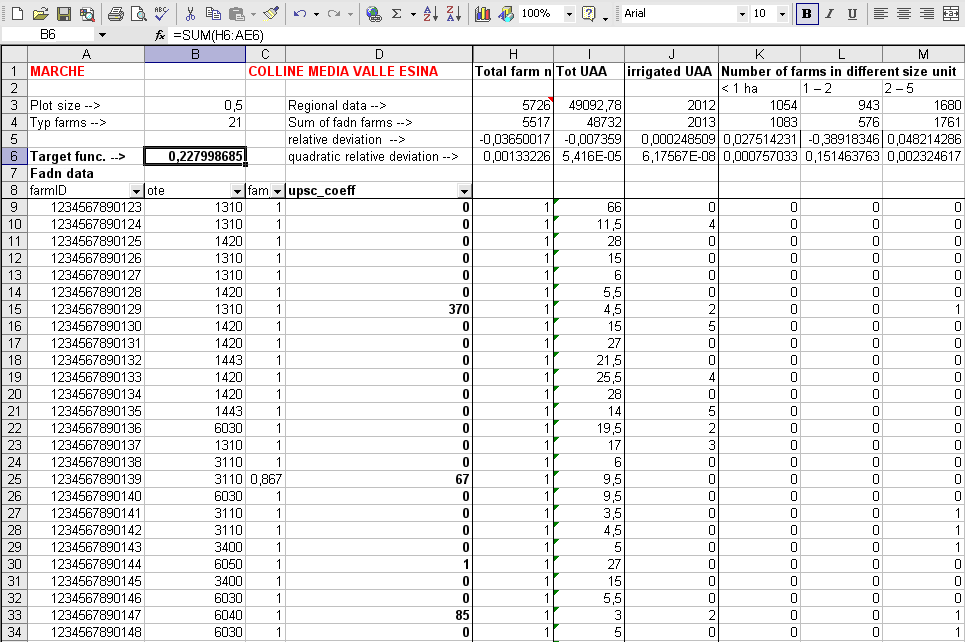
\includegraphics[width=\textwidth]{imgs/upscalingMatrix.png}
	\label{fig:upscaling}
\end{figure}

\section{Advanced: changing RegMAS structure}
\label{sec:programming}
If agents should behave in a different way that the default one (profit maximisation), or if the model should work with more agent types, RegMAS needs to be modified to achieve such tasks.

It doesn't yet provide a plug-in architecture, so changes have to be done directly in its source tree.
However the design is made in a way to separate as much as possible the core model logic from those of the agents.
The logic of the agents is described by two main classes: \texttt{Manager\_base} and \texttt{Agent\_base}. The former is the agent-side interface with the model, and manages the behaviour of the individual agents (that are instances of the latter class).
As the name suggests, they are base classes that are derived in more specialised classes, like \texttt{Agent\_space} and \texttt{Agent\_farmer}.

The equivalent interface at the model-side is \texttt{SuperAgentManager} and there is only one instance of this class. It doesn't know anything of individual agents, as its relationship is only with the different managers.

The model run sequentially following two main functions: \texttt{Init::setInit\\Level()} during initialisation stage and \texttt{Scheduler::run()} during simulation.
The latter function performs a loop for each iteration that is due (see the Flowchart, Fig. \ref{fig:flowchart})


Other important classes are those managing the regional data (\texttt{RegData}), the model objects (\texttt{ModelObject}) the regional level activities and resources (respectivelly \texttt{RegActivities} and \texttt{RegResources}) and finally the optimisation problem associated to each agent (\texttt{Opt}).

All classes are documented in the Reference Manual that is build directly from the source code using Doxygen.

RegMAS is know to compile using Gcc on both Linux and Windows. In the CVS a \textit{project file} is provided for two user-friendly Integrated Development Environment (IDE) for both the OSes, KDevelop and Dev-C++.
Using one of this two IDE is strongly recommended, as fully tested.

Source code is available under the GPL license, see the appendix for details.

\section{Model output}
\label{sec:results}
The verbosity of the output can be set through the \textit{outputLevel} parameter, from 0 (no output) to 7 (all possible outputs).

In the middle, option 3 will print yearly maps for each layer and aggregated regional data (including data for leaving farms) and option 5 adds individual agents data.

With option 7 it is also possible to print the matrices comprising the mixed-integer problem that agents need to solve in order to ``produce'' in the model.

Furthermore it is possible to decide if having a fully deterministic model, or - changing the seed of the random number generator with the \textit{randomSimulation} option - allow for a stochastic simulation.

\subsection{Spatial results}
As RegMAS is spatially explicit any information in the model with a spatial attribute can be printed as a map, e.g. for further elaboration with a GIS (see next section).

Available maps are the farms location, their rented and owned plots, their spatial activities (e.g. durum wheat) and the overall agricultural usage. The last one allows users to have a quick view of abandoned land.

Maps are exported as ArcINFO or GRASS ASCII grids and from RegMAS version 1.0 RC2 they can be exported directly as images (.png files).

\subsection{Quantitative results}
On each simulation year, RegMAS can produces a very large amount of data, as shown on Table \ref{tab:resultsType}.

\begin{table}[!h]
	\begin{threeparttable}
	\centering
	\caption{Result categories}

\begin{tabular}{l l}
\hline
\textbf{Aggregated results} & \textbf{Individual agent results} \\
\hline
(Sum) of Agents by type   & Agent type    \\
                        & Agent ID      \\
                        & Agent Mould ID \\
                        & Host plot ID \& coordinates \\
(Avg) Total, land and object capitals & Total, land and object Capitals \\
(Avg) Profit             & Production profit \\
(Avg) Coupled premiums   & Coupled premiums \\
(Avg) Decoupled premium  & Decoupled premium (SFP) \\
(Avg) Sunk costs         & Sunk cost paid \\
(Sum) Rental land prices by type & \\
(Sum) Abandoned and idle plots by type & \\
(Sum) Owned plots by type     & Owned plots by type \\
(Sum) Rented plots by type    & Rented plots by type \\
                        & Owned objects by type\\
(Sum) Available objects by type & Available objects by type \\
(Sum) New investments by type & New investments by type \\
(Sum) Production activities by type      & Production activities by type \\


\hline
\end{tabular}
%\begin{footnotesize}Source: Reg. 1782/2003\end{footnotesize}
\label{tab:resultsType} 
\end{threeparttable}
\end{table}

Furthermore similar results are available for farmers that leave the agricultural sector.

Most data is collected trough a ``survey'' that each agent is asked to fill, more or less how it happens with real statistics.

Rental prices are updated from the previous year (or, on the first year, from initial renting prices) only if in the model there are at least 5 new contracts for that specific soil type.

Abandoned plots sum two different kind of plots: those owned or rented by an existing farm but not utilised at all, and those owned by a farm that left the model and that are srill unrented.

The difference in the detailed data between owned and available objects is due to the fact that agents may have rented plots including spatial objects that are not in their property basket but that thanks to the renting contract become available to their production activities: the formers are important in the capital formation, the latter to the production decisions.

On both the aggregated and the detailed results the ``activities by type'' values refer to the results arising form the solution of the agents profit-optimisation problem.

\section{Exporting results to a Geographical Information System}
\label{sec:gis}
Under the \textit{output/map} folder a couple of scripts are provided to automatise the importing of RegMAS results into the GRASS GIS.

Although quite irksome to learn, Grass GIS is a very powerful open source multi platform desktop GIS that is particularly suited for raster spatial analysis and, even more important, is fully scriptable.
Users can read more of it on its web-site\footnote{\url{http://grass.itc.it/}} or it can be downloaded it in bundle qith QGis \footnote{\url{http://www.qgis.org}}, a gis application that wrap Grass making it much more easy to be used.

To import spatial data inside a GIS program manually, users have to import the raw data, define the categories and pick-up the colour for each category. These are located respectively under the \textit{asciiGrid}, \textit{cats} and \textit{colr} subfolders. Furthermore an empty ``Region'' in the Grass format is provided in the \textit{grass/ColliEsini} subfolder, containing a ``skeleton'' structure (e.g. the geographic coordinated) for the sample region.

Under Linux or Windows/Cygwin environment, the \textit{importInGrass.sh} script will does the import automatically (calling the second script \textit{runWithinGrass.sh} to invoke Grass commands) otherwise individual maps can be imported from the Grass command \textit{r.in.ascii} and then the associated category and colour description files should be copied in the working region.

GIS post-processing is useful when we want to place into relation several spatial data, e.g. in order to calculate the land abandonment, or the production intensity or even the farm density by elevation zone or by soil type.

We could also build a matrix to show which productions are switched to an other production type after a policy change.

Plans are to create a repository of scripts to produce such statistics from the RegMAS output and user submission of their own scripts is welcome.

%\section{Exporting to MySQL}
%./csv2sql.py ==> generate detailedResults_adj.csv (include record ID)
%mysql -l
%use <DABASENAME>
%load data infile '<FULLPATH>' into table <TABLE_NAME> fields terminated by ';'; 

\newpage
\bibliography{biblio}


\appendix

\section{Getting help}
\label{sec:getting_help}

RegMAS documentation is organised on three main levels.

\begin{itemize}
\item The \textbf{Official Documentation} includes the \textit{User Manual} (this document) and the \textit{Reference Manual}.
The former introduce the program and present the tasks that users needs to accomplish to run their own simulation. The latter is instead addressed to advanced users with programming experience. It is automatically generated from the source code using the Doxygen tool and describes the classes that compose ReGMAS and how they are related.
\item The \textbf{Contributed Documentation} is instead organised as a \textit{wiki}, where users can find (and possibly, contribute) on specific topics. Contributed documentation does not claim to be well-organised and completed like the official documentation, but includes specific topics that are not documented in any other place (e.g. how the agents decision matrix is composed).
\item Finally the \textbf{Community Project} (hosted at SourceForge) includes a forum and a mailing-list for discussions and a tracking system to report bugs, wish-list, to-do etc..
\end{itemize}

All documentation is available from the url \url{http://www.regmas.org/doc}.

% Both RegMAS and this User Manual are at their very initial stage.
% 
% Depending on your needs you can find several source of documentation.
% 
% The documentation\footnote{\url{http://www.regmas.org/doc}} is organized according to the user needs.
% For users that are interested in the simulation of the social system, you can also refer to the documents cited on section \ref{sec:methodology} and for those that want understand the code we use doxygen-generated documentation\footnote{\url{http://www.regmas.org/doc/api/html}}.
% 
% A forum and a bug reporting system is also available.


%\section{Classes collaboration diagrams}
%\label{sec:api}
%Main classes of regmas with:
%- collaboration diagrams
%- members
%- brief descriptions

%\include{../autogeneratedDoc/latex/classAgent__base}
%\input{../autogeneratedDoc/latex/classAgent__base}

\section{Licence}
\label{sec:licence}
\subsection{GPL}
%\verbatimtabinput[4]{../../COPYING} % include a text file converting tabs in 4 spaces
RegMAS is released under the GNU General Public License, Version 3 (GPL).

A copy of such licence is always enclosed with any release of the software and can also be obtained from \url{http://regmas.org/cgi-bin/viewvc.cgi/regmas/COPYING?view=co}.

In shorts, RegMAS can be copied and it is freely modified to produce derivative work, as long as the licence terms of the derivative work doesn't change and the source code (including those of the derivative work) remains publicly available.

%\subsection{Citing RegMAS derived works}
%Citing RegMAS in your results is not legally required.

\end{document}
